
\begin{frame}
  \frametitle{Ehad and the Big Finale -- solución}

  Nos paramos en la raíz y vamos bajando hasta llegar a \(\star\), sin salirnos del camino de los ancestros de \(\star\) (para poder usar la consulta \texttt{s}).

  \vspace{0.75em}

  La idea del algoritmo es ir caminando de la raíz hasta \(\star\), pero saltando de un camino pesado al siguiente en cada paso: si estamos en un camino pesado, saltar rápido a la posición en la que el camino hacia \(\star\) se sale del camino pesado.
\end{frame}

\begin{frame}
  \frametitle{Consultas \texttt{d} en un camino pesado}

  Al estar en un camino pesado podemos hacer 2 consultas \texttt{d}(-):
  \begin{itemize}
    \item una en el nodo de arriba de todo (\(u\)),
    \item otra en el de abajo de todo (\(v\)).
  \end{itemize}

  \vspace{0.75em}

  Al saber las distancias \(u\text{-}\star\) y \(v\text{-}\star\), y la distancia \(u\text{-}v\), podemos calcular el punto en el que el camino raíz-\(\star\) se sale del camino pesado \(u\text{-}v\).
\end{frame}

\begin{frame}
  \frametitle{Localizar la salida con \texttt{d}(u) y \texttt{d}(v)}

  \centering
  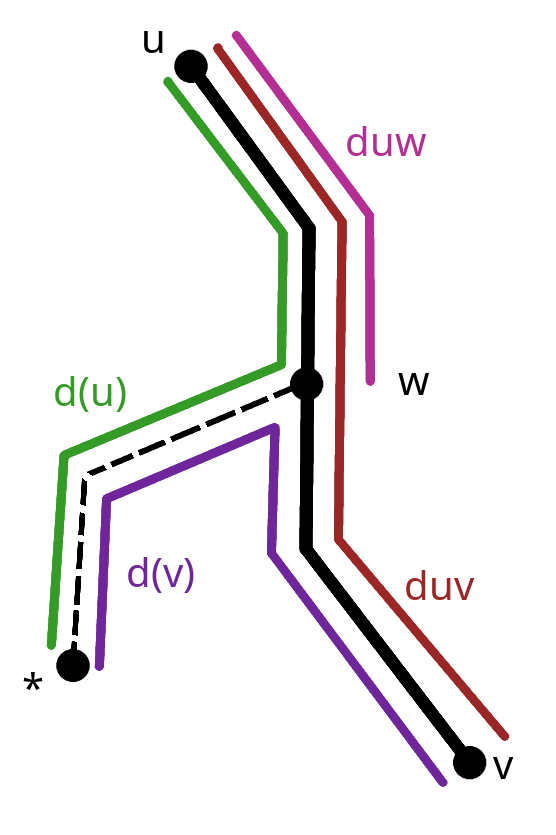
\includegraphics[height=0.55\textheight,keepaspectratio]{fotos/jumps.png}

  \vspace{0.4em}

  \[
    \text{duw} = \frac{duv + d(u) - d(v)}{2}
  \]

\end{frame}

\begin{frame}
  \frametitle{Cruzar la arista liviana}

  Una vez que sabemos el punto en el que se sale, sabemos que ahí hay que cruzar una arista liviana, pero no sabemos cuál.

  \vspace{0.75em}

  Para resolver eso hacemos una consulta \texttt{s}(-).

  \vspace{0.75em}

  Como nos mantenemos siempre en un camino nodo-raíz, la cantidad de aristas livianas y caminos pesados que tocamos es a lo sumo \(\log_2(N)\).

  \vspace{0.75em}

  Ahí tenemos una solución en \(3\log(N)\) consultas.
\end{frame}

\begin{frame}
  \frametitle{Optimización a \(2\log(N)+1\)}

  Se puede optimizar a \(2\log(N)+1\) evitando hacer consultas \texttt{d} en el nodo \(u\) en cada camino pesado: hacemos una consulta \texttt{d(raíz)} al principio y por cada paso que damos le restamos uno.
\end{frame}

\begin{frame}[fragile,shrink=5]
  \frametitle{Código: \texttt{special()}}

\begin{lstlisting}[basicstyle=\ttfamily\scriptsize]




                    int special() {
                        int u = 0;
                        int du = d(u);
                        while (true) {
                            if (du == 0) return u;
                            int duv = 0;
                            int v = u;
                            while (h[v] != -1) v = h[v], duv += 1;
                            int dv = d(v);
                            int steps = (du - dv + duv) / 2;
                            forn(_, steps) u = h[u], du -= 1;
                            if (du == 0) return u;
                            u = s(u);
                            du -= 1;
                        }
                    }
\end{lstlisting}
\end{frame}
